\chapter{Svolgimento stage}
\label{cap:svolgimentoStage}
In questo capitolo vengono descritte tutte le attività da me svolte durante lo \emph{stage}, divise nelle sezioni “Analisi”, “Progettazione”, “Programmazione” e “Verifica e validazione”, in modo da fornire una panoramica chiara e strutturata del lavoro svolto, evidenziando il processo seguito e le competenze acquisite in ciascuna fase.\\
Esse non sono intese come completamente sequenziali bensì, fin dalla prima fase, sono presenti tutte le attività correlate in modo da coprire l'intero periodo di \emph{stage}.\\
\section{Analisi}
In questa sezione sono presenti tutte le attività analitiche da me svolte e il suo scopo è descrivere le modalità con cui ho compreso i bisogni e i requisiti del mio progetto di \emph{stage}. 

\subsection{Requisiti}
Gli obiettivi del mio \emph{stage}, come dichiarati nel documento “Progetto Formativo” generato all'inizio del suo svolgimento, sono divisi in categorie:
\begin{enumerate}
	\item[O -]requisiti obbligatori, vincolanti in quanto obiettivi primari richiesti dall'azienda.
    \item[D -]requisiti desiderabili, non strettamente necessari ma dal riconoscibile valore aggiunto.
    \item[F -]requisiti facoltativi / opzionali, rappresentanti un valore aggiunto non strettamente competitivo.\\
\end{enumerate}

Essi sono:
\begin{table}[htbp]
    \label{tab:obiettiviProgettuali}
    \renewcommand{\arraystretch}{1.5}
    \begin{tabularx}{\textwidth}{|l|X|l|}
    \hline
    \textbf{Codice} & \textbf{Descrizione}\\
    \hline
    O1    & Mappatura delle funzionalità possibili tramite l'adozione dei due applicativi \gls{Sistemi} e Office365.\\
    \hline O1.1  & Analisi approfondita del sistema e delle parti interessate.\\
    \hline O1.2  & Studio delle modalità di lavoro degli utenti.\\
    \hline O1.3  & Produzione di una completa documentazione di uso.\\
    \hline O2  & Personalizzazione e integrazione: individuare le modalità di utilizzo.\\
    \hline
    \hline D1  & Analisi dei requisiti per l'integrazione aziendale della metodologia \gls{DevOps} in ambito \GLS{Sistemi} e Office365.\\
    \hline D2  & Produzione di una completa documentazione progettuale.\\
    \hline
    \hline F1  & Realizzazione di \emph{Proof of concept}.\\
    \hline F2  & Presentazione interna.\\
    \hline F3  & Predisposizione della documentazione.\\
    \hline
    \end{tabularx}
    \caption{Tabella degli obiettivi progettuali.}
\end{table}%
\subsection{Ambiente di lavoro}
Durante i primi giorni dello \emph{stage} sono stato introdotto all'ambiente di lavoro e alle tecnologie di comunicazione e collaborazione.\\
Conseguentemente ho analizzato e utilizzato il sistema di messaggistica basato su Microsoft Teams e Outlook e ho compreso la struttura di condivisione dei dati, utilizzata in azienda, basata sullo strumento Microsoft SharePoint.\\
Esso è una piattaforma \emph{software} in grado di organizzare dati sottoforma di \emph{file} e strutture tabellari chiamate “Liste”, al fine di gestire il materiale condiviso dall'azienda e dai singoli \emph{team} tramite un sistema di accessi e autorizzazioni.\\


Tramite questi strumenti ho studiato i documenti aziendali a me forniti in modo da comprendere i principali processi produttivi di Wintech.\\ 
Tali documenti comprendono i “Documenti di sviluppo sicuro” e includono:
\begin{itemize}
    \item Agile e SCRUM: descrizione delle metodologie Agile e SCRUM, spiegazione dei ruoli necessari e delle cerimonie previste. 
    \item Presentazione sviluppo sicuro: presentazione PowerPoint atta a descrivere i processi aziendali atti a migliorare la qualità dei prodotti realizzati automatizzando fasi ripetitive e rispettando criteri di sicurezza. 
    \item Modelli di sviluppo sicuro: elenco dettagliato dei documenti di sviluppo sicuro i quali descrivono come applicare automazioni processuali (per esempio i processi di \emph{build} e \emph{deploy}) in modo sicuro e normato. 
    \item Politiche di sviluppo sicuro: strategie e normative aziendali definite al fine di garantire sicurezza e qualità nei processi e nel ciclo di vita del \emph{software}. 
    \item Piani di progetto degli altri stagisti: piani formativi degli altri due stagisti che nel mio stesso periodo hanno effettuato lo \emph{stage} universitario in Wintech. 
\end{itemize}
Relativamente a quest'ultimo punto, nei primi giorni ho approfondito il lavoro svolto dagli altri stagisti tramite appositi \emph{meeting} nei quali mi hanno descritto i risultati ottenuti fino a quel momento. Essi, avendo iniziato lo svolgimento del progetto circa una settimana prima, mi hanno esposto, mediante apposite presentazioni PowerPoint, le proprie ricerche riguardanti l'utilizzo dello strumento Git e dello studio avvenuto riguardo la possibilità di integrare tra loro gli strumenti Planner e Taiga. 

\subsection{Requisiti progettuali}
Dopo aver compreso le tecnologie e i principali processi aziendali, ho partecipato ad un \emph{meeting} con il \emph{tutor} aziendale al fine di discutere il mio progetto di \emph{stage}.\\
I requisiti scaturiti da tale incontro sono stati: 
\begin{itemize}
    \item Autoapprendimento dello strumento Power Automate.
    \item Realizzazione di un PoC che testasse la possibilità di realizzare un flusso approvativo Power Automate. 
    \item Testare le funzionalità disponibili con le licenze di utilizzo \emph{standard}. 
\end{itemize}

\subsubsection*{Power Automate}
Ho pertanto studiato approfonditamente tali tecnologie con l'ausilio delle numerose guide e \emph{tutorial} offerti da Microsoft. 
Essi sono direttamente accessibili dalla \emph{home} di Power Automate e Power Apps e sono divisi in moduli testuali corredati da immagini, dalla durata e argomenti specifici. 

\begin{figure}[htbp] 
    \centering 
    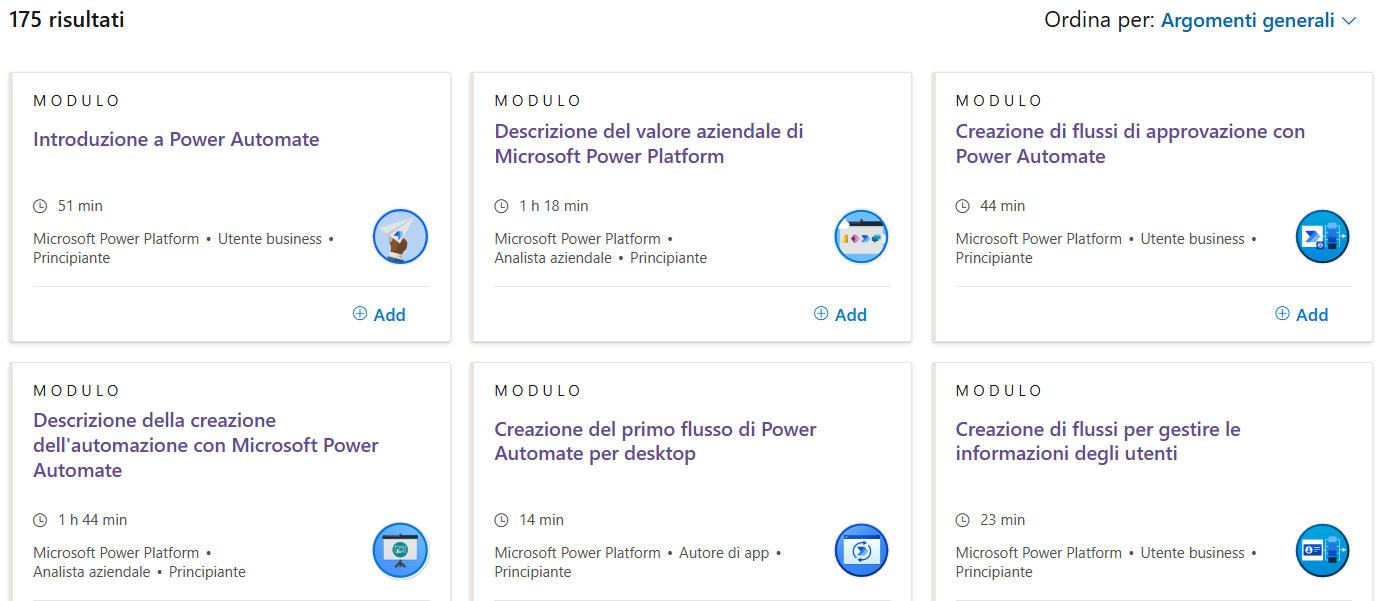
\includegraphics[width=1\columnwidth]{moduliPowerAutomate} 
    \caption{Moduli formativi per Power Automate.}
    \label{fig:moduliPowerAutomate}
    \vspace{1mm}
    Fonte: \url{https://learn.microsoft.com/it-it/training/browse/?products=power-automate}.
\end{figure}

Lo studio di tali moduli mi ha permesso di comprendere il funzionamento e le \emph{features} principali di Power Automate:\\
Esso è formato da una pagina web che offre controllo sui flussi di automazione creati: è possibile modificarli e visualizzarne i dettagli, le esecuzioni e le statistiche. È possibile creare dei nuovi flussi partendo da altri progetti pubblici, o a noi condivisi, e modelli offerti da Microsoft da adattare alle proprie esigenze.\\
La modifica di un flusso non avviene mediante la scrittura di codice tramite un linguaggio di programmazione bensì tramite una composizione “a blocchi” personalizzabili collegati tra loro ciascuno avente proprietà e attributi definiti.\\
Essi sono selezionabili da una lista di blocchi relativi ciascuno a una funzionalità specifica di un servizio Microsoft.\\
Tali blocchi possono essere “Trigger” o “Azioni” ed entrambi sono necessari per la creazione e il funzionamento di un flusso.\\ 
In ogni flusso è presente uno e un solo Trigger il quale rappresenta il suo punto di partenza nonché la condizione che scaturisce la sua esecuzione.\\
Esistono tre tipologie principali di Trigger le quali determinano la tipologia stessa di ogni flusso:
\begin{itemize}
    \item Automatico: per esempio “SharePoint - Quando viene creato un elemento”. 
    \item Istantaneo: per esempio “Attiva manualmente un flusso”.
    \item Pianificato: per esempio “Ricorrenza”, il quale attiva il flusso periodicamente.\\
\end{itemize}

\noindent Ad ogni Trigger possono essere collegate, in serie o in parallelo, una moltitudine di Azioni, ciascuna responsabile di uno specifico compito, per esempio sono presenti le azioni “Inizializza variabile”, “Avvia e attendi un'approvazione”, “Teams - Crea una chat” e “OneDrive - Crea file”.\\
Sono inoltre presenti azioni dedicate alla gestione logica dei flussi come “Condizione" e “Do until”. La prima rappresenta la struttura di controllo rappresentata nei classici linguaggi di programmazione con “if”, responsabile della ramificazione dell'esecuzione del flusso in base a una condizione specifica.\\
La seconda rappresenta la struttura di controllo rappresentata nei classici linguaggi di programmazione con “Do while”, responsabile della ripetizione condizionata di un insieme di azioni garantendone sempre la prima esecuzione.\\

/// immagine esempio di flusso/// 

\noindent Successivamente è emersa, da parte del tutor aziendale, la necessità di integrare i flussi Power Automate con il \emph{software} gestionale WOW e gli altri prodotti aziendali al fine di poter integrare le funzionalità desiderate con libertà mantenendo coordinate le diverse parti del prodotto.\\
Sono emersi quindi due requisiti: il primo, utile per apprendere le tecnologie in oggetto, è relativo alla creazione di un flusso che automatizzasse un processo approvativo.\\
Il secondo, più concreto e integrabile con i prodotti aziendali, è basato sull'applicazione, ai flussi Power Automate, di chiamate \gls{http}(Hypertext Transfer Protocol): in italiano “protocollo di trasferimento ipertestuale” è un protocollo di rete, ovvero un insieme di regole formalmente descritte che definiscono le modalità di comunicazione tra due o più apparecchiature elettroniche, usato come principale sistema per la trasmissione d'informazioni sul web.\\
Esse permettono la comunicazione e lo scambio di dati tra flussi Power Automate e altri flussi o applicazioni: esiste infatti la possibilità di richiamare lo specifico Trigger “Alla ricezione di una richiesta HTTP” il quale genera un personale URL (Uniform Resource Locator), ovvero una sequenza di caratteri che identifica univocamente l'indirizzo di una risorsa su una rete di computer.\\
In seguito è possibile utilizzare la corrispondente azione “Response” al fine di rispondere al chiamante con l'output della richiesta.\\

\subsection{DevOps}
\subsubsection*{Plan}
\subsubsection*{Code}
\subsubsection*{Build}
\subsubsection*{Test}
\subsubsection*{Release}
\subsubsection*{Deploy}
\subsubsection*{Operate}
\subsubsection*{Monitor}

\section{Progettazione}
In questa sezione sono presenti tutte le attività progettuali da me svolte e Il suo scopo è descrivere le modalità con cui ho individuato le soluzioni ai bisogni progettuali in modo da soddisfarne i requisiti.

\section{Programmazione}
In questa sezione sono presenti tutte le attività da me svolte al fine di sviluppare e implementare le soluzioni individuate in fase di progettazione.

\section{Verifica e Validazione}
In questa sezione sono presenti tutte le attività da me svolte al fine di verificare il corretto funzionamento delle soluzioni sviluppate e il loro soddisfacimento dei requisiti progettuali.

\section{Risultati raggiunti}
\subsection{Qualitativamente}
%

\subsection{Quantitativamente}
%
